\documentclass{article}

\usepackage[margin=1in]{geometry}
\usepackage[center]{caption}
\usepackage{subfigure}
\usepackage{appendix}
\usepackage{amsmath}
\usepackage{graphicx}
\usepackage{todonotes}
\usepackage{tikz}
\usetikzlibrary{fit,positioning}
\usepackage{verbatim}
\usepackage{float}
\usepackage{placeins}
\usepackage{color,soul}
\usepackage{framed}

\newcommand{\HRule}{\rule{\linewidth}{0.1mm}}
\newcommand{\code}[1]{\texttt{#1}}

% dit is voor twee plaatjes naast elkaar 
%-----------------------
\newcommand{\twopicsf}{
	\begingroup
  	\catcode`_=12 
  	\triplet
}
\newcommand{\twopics}[6]{
	\begingroup
		\begin{figure}[htbp]
			\centering			
		      	\subcaptionbox{#1}[70mm]{\includegraphics[width=0.5\textwidth]{#2}}    
		  	\hspace{10mm}  
		      	\subcaptionbox{#3}[70mm]{\includegraphics[width=0.5\textwidth]{#4}}   		   
		    \hspace{1mm}
		  	\caption{#5}
		  	\label{#6}
		\end{figure}		
	\endgroup
}
%-----------------------

\begin{document}

\title{ \HRule \\[0.2cm]
		Autonomous Agents\\ 
		Report Assignment 3: Multi-Agent Planning and Learning\\
		\HRule \\[0.1cm]
		}
		
\author{
		\emph{Authors:}\\[0.2cm]
		Agnes \textsc{van Belle} \small{ \emph{(10363130)}},\\ 
		Maaike \textsc{Fleuren} \small{ \emph{(10350470)}}, \\
		Norbert \textsc{Heijne} \small{ \emph{(10357769)}}, \\
		Lydia \textsc{Mennes} \small{ \emph{(10333843)}}
		}
		
\maketitle


\section{Introduction}
This report has been written for the Master Artificial Intelligence course Autonomous Agents. This report will contain the answers, motivation and explanation for our implementations of the tasks we had to accomplish in our third assignment for this course. These tasks were centered around the topic of `Multi-Agent Planning and Learning'.

\subsection{The environment} \label{sec:environment}
In all tasks there is assumed to be a grid world (of $11 \times 11$) with at least one predator and a prey in it. The agents can both move one tile forward each iteration. The direction they take (or if they move at all) is affected by probabilities (their policies). If they move over the edge of the grid they end up at the opposing side of the grid. We are focused on improving the decisions of all the agents, the predator(s) and the prey. 

\subsection{The state space representation} \label{sec:stateSpace}
In the experiments described the first report, we initially used a state space that was an intuitive, yet cumbersome representation. We referred to that state space representation as the `default' state space. The amount of states that was used in the default state space was $(11 \times 11) \times (11 \times 11) = 121 \times 121 = 14641$. We then changed the state space representation to a more efficient one in the second assignment, referred to as the `efficient' state space, which led to a reduction of 697 times less states, resulting in just 21 different states.
The default amount of states for four predators and a prey would be $121^(p+prey)$


In this assignment, we again used this efficient state space representation for the learning algorithms. To give a good understanding of our learning algorithms, which were built on the efficient state space representation, we will once again explain how this representation works.

Figure \ref{fig:statespaceSymm} illustrates that there is a symmetry in the default state space, and thus that there were relatively much values redundantly computed.
By using this symmetry in the default state space a much smaller state space was achieved. 

Each state represents a distance between the prey and predator. These are represented in the lower left diagonal of a matrix, in which the $x$-axis is the relative horizontal distance in the MDP and the $y$-axis the relative vertical distance in the MDP. This matrix is shown in Figure \ref{fig:NewStateRep}. Combinations of positions of prey and predator for which the horizontal and vertical distances are equal are now treated equivalent. 
Also two combinations for which the horizontal distance in one equals the vertical distance in the other and vice versa are considered equal. In order to navigate through this state space different actions are required. These are: \textit{horizontal retreat, horizontal approach, vertical retreat, vertical approach}, as illustrated in Figure \ref{fig:statespaceSymm}, and of course the action \textit{wait}. When interacting with the environment these actions are converted into corresponding actions in the real world. This only requires the relative direction of the prey (which is always located at the centre, regardless of its coordinates) with respect to the predator. This is computed by using the difference in location of the prey and predator on the $x$- and $y$-axis.

\begin{figure}[ht]
\centering
\subfigure[The $11 \times 11$ grid divided into eight symmetric pieces, with the corresponding possible moves which are also symmetric.]{
    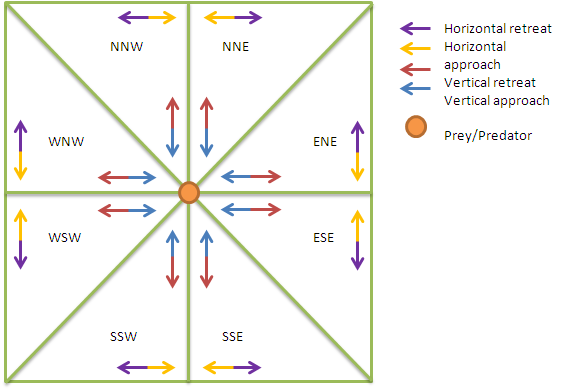
\includegraphics[width=0.5\textwidth]{statespaceSymm.png}
    \label{fig:statespaceSymm}
}
\subfigure[Colormap of $V$-values, the brighter the color the higher the corresponding $V$-value. The prey is always located on the (1, 1) coordinate in this state representation.]{
    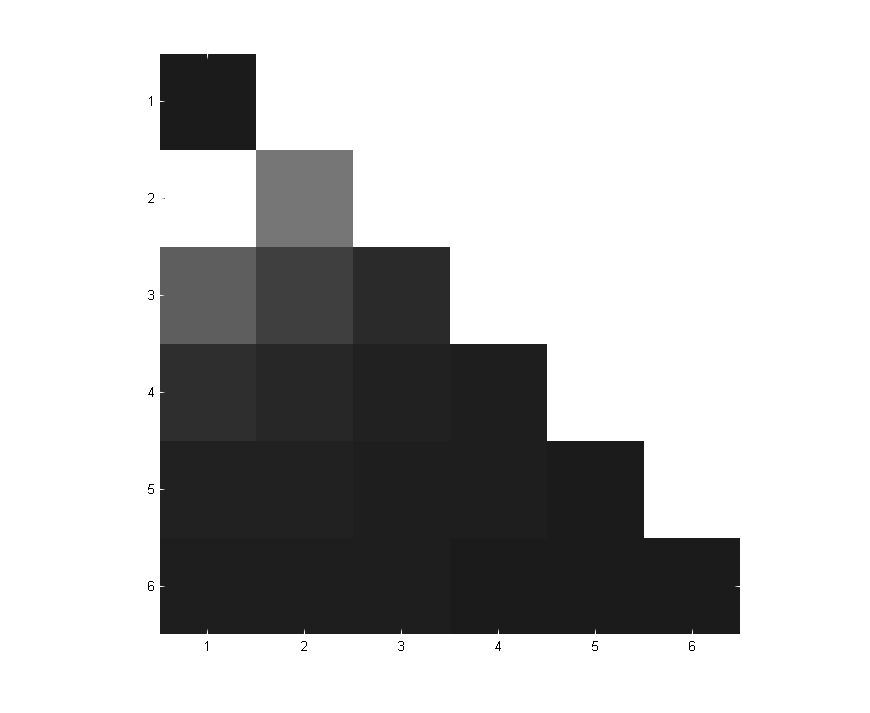
\includegraphics[width=0.4\textwidth]{VMatrixNewStateRep.png}
    \label{fig:NewStateRep}
}
\caption{Illustration of the symmetry and corresponding values of the new state space representation}
\label{fig:statespaceIll}
\end{figure}


\subsection{Implementation details}
This report will not be about our exact code and implementation details. However, a class diagram of our code is provided in Appendix \ref{app:classDiagram}.


\newpage
\section{Independent Q-Learning}\label{sec:IQL}
Q-Learning is an off-policy temporal difference control algorithm. Temporal difference methods can learn directly from raw experience without a model of the environment's dynamics. Furthermore, it updates estimates based in part on other learned estimates, without waiting for a final outcome \cite[pp. 133]{RL1}. 

While the distinguishing feature of on-policy methods is that they estimate the value of a policy while using it for control, these two functions are separated in off-policy methods. The behavior policy, used to generate behavior, and the estimation policy, that is evaluated and improved, may in fact be unrelated. This separation is an advantage because the estimation policy may be deterministic (e.g., greedy), while the behavior policy can continue to sample all possible actions \cite[pp. 126]{RL1}. Its simplest form, \emph{one-step Q-learning}, is defined by \cite[pp. 148]{RL1}:
\begin{align*}
Q(s_t,a_t) & \leftarrow Q(s_t,a_t) + \alpha \left[ r_{t+1} + \gamma \displaystyle\max_a Q(s_{t+1},a) - Q(s_t,a_t) \right]
\end{align*}
When using Q-Learning in a multi-agent setting independently for each agent, the method is called Independent Q-Learning (IQL). In IQL, for a single agent, all the other agents are modeled as part of the environment. While Q-Learning is guaranteed to converge, Independent Q-Learning is not guaranteed to converge. This is because the premise of the convergence porperty of Q-Learning is that the environment be stationary. This will not be the case in a multiagent setting in which agents are learning concurrently, since the agents base their policy upon the movements of the other agents which are also learning. That is, the other agents don't act deterministically but are modeled as such. Independent Q-Learning can thus not be justified theoretically \cite[pp. 57]{vlassis}.

\subsection{Implementation}
For this assignment, we implemented Independent Q-learning and used it independently for all our agents, the predators and the prey. The agents learn concurrently (i.e. all agents do a move, then all update their estimated values), not sequentially (i.e. after one agent does a move, all other agents update their estimated values). When any two predators bump into each other, the prey wins (reward of $10$) and the predators all lose (reward of $-10$). When a predator catches the prey, the prey loses and all predators win.

 Each agent will have its own state representation and learning and will view the other agents as part of the environment. We used $\epsilon$-greedy action selection, which behaves greedily most of the time, but with probability $\epsilon$, instead select an action at random, uniformly, independently of the action-value estimates \cite[pp. 28]{RL1}. In this case, we used $\epsilon = 0.1$. We initiated the values of each Q-learning table optimistically with a value of 15 for all cells for the tables. Furthermore the learning rate $\alpha$ was set to 0.5 and the discount factor $\gamma$ was set to 0.9.

\subsubsection{State space} \label{sec:stateSpaceIQL}
The state space is of crucial importance to Independent Q-Learning, because it grows exponentially with the number of agents. In the experiments described in the previous report, were we had just one prey and one predator, we initially used a state space that was an intuitive, yet cumbersome representation. We then changed the state space representation to a more efficient one in the second assignment, referred to as the `efficient' state space, which led to a reduction of 697 times less states, resulting in just 21 different states. See Section \ref{sec:stateSpaceIntro} for details.

The default amount of states for this assignment would be $121^{p+1}$ for each agent, where p equals the number of predators. By using the efficient state space this has been reduced to $21\cdot 121^{p-1}$ because the prey's position is fixed in the state space representation and the predator to which this state space belongs moves along those $21$ states, the rest is used to determine in which state the predator currently resides. In this assignment however the prey also learns, so to make use of our state space representation, a single predator will be used as reference point every time so that the predator is fixed at the position $(0, 0)$ in our state space and the prey would be moving around the $21$ states just like a predator. 

The reduction is increased further by pointing to the same state for each combination of current positions of the other predators, though this is only effective for more than two predators. A simple example would be a case three predators and a prey, the current predator ($p_1$) which has to find his current state would take the position of the first other predator ($p_2$) and then the position of the second other predator ($p_3$) to locate his state in the state space. In this case it shouldn't matter which position, $p_2$ or $p_3$, would be looked up first. In this case both $p_2$ then $p_3$ and $p_3$ then $p_2$ would point to the same state. This reduces the state space to:

\[
\mathbf{stateSpaceSize}(p) = 
\begin{cases}
	21 & p = 1\\
    21 \cdot 121 & p = 2 \\
    \frac{21\cdot 121^{p-1}}{(p-1)!}& p > 2
\end{cases}
\]


\subsection{Results}

We analyzed what happened in the case of 2, 3 and 4 predators.
For the case of one predator (and one prey), we have not used this case here, we used this case in the comparison with the Minimax-Q algorithm (in Section \ref{sec:comparisonIQLandMinimax}).

After producing the results it came to our attention that Q-learning did not yet have the prey trip chance implemented, for more than one predator it did not cause an infinite loop (the predators' policies were good enough to catch a prey that cannot trip). However, for the results in Section \ref{sec:comparisonIQLandMinimax}  this was implemented, where before it would cause the prey to stay away from a single predator indefinitely.

Even though we were using an efficient state space representation we ran out of time while trying to initialize one prey and four predators for the $11 \times 11$ grid world. We dedicated around $3.6$ GB heap space for the JVM on a $64$-bit machine with $4$ processor cores of $2.67$ Ghz, and under these settings it took more than $7$ hours to declare and initialize four predators, the prey not being created and initialized yet.
However, when using a $9 \times 9$ grid world instead of a $11 \times 11$ one, the five agents were in short time up and running. 
Therefore we will show the results for $2$, $3$ and $4$ predators for this $9 \times 9$
 grid world first, and later we will attempt to make a comparison with the $11 \times 11$ grid world.



\subsubsection{Number of predators}\label{sec:IQLresults1}
We kept track of two measures:
\begin{itemize}
\item The number of time steps before the game was ended (by collision or catching)
\item If the predators won the episode, or not 
\end{itemize}
We ran each episode $\mathbf{200}$ times. Therefore these measures are displayed as an average value and a percentage value, respectively.

In Figure \ref{fig:IQLmeansSds} are the means and standard deviations shown for a total of $5000$ episodes, for the different numbers of predators.

\begin{figure}[htb]
\centering
%bb = llx, lly, urx, and ury;
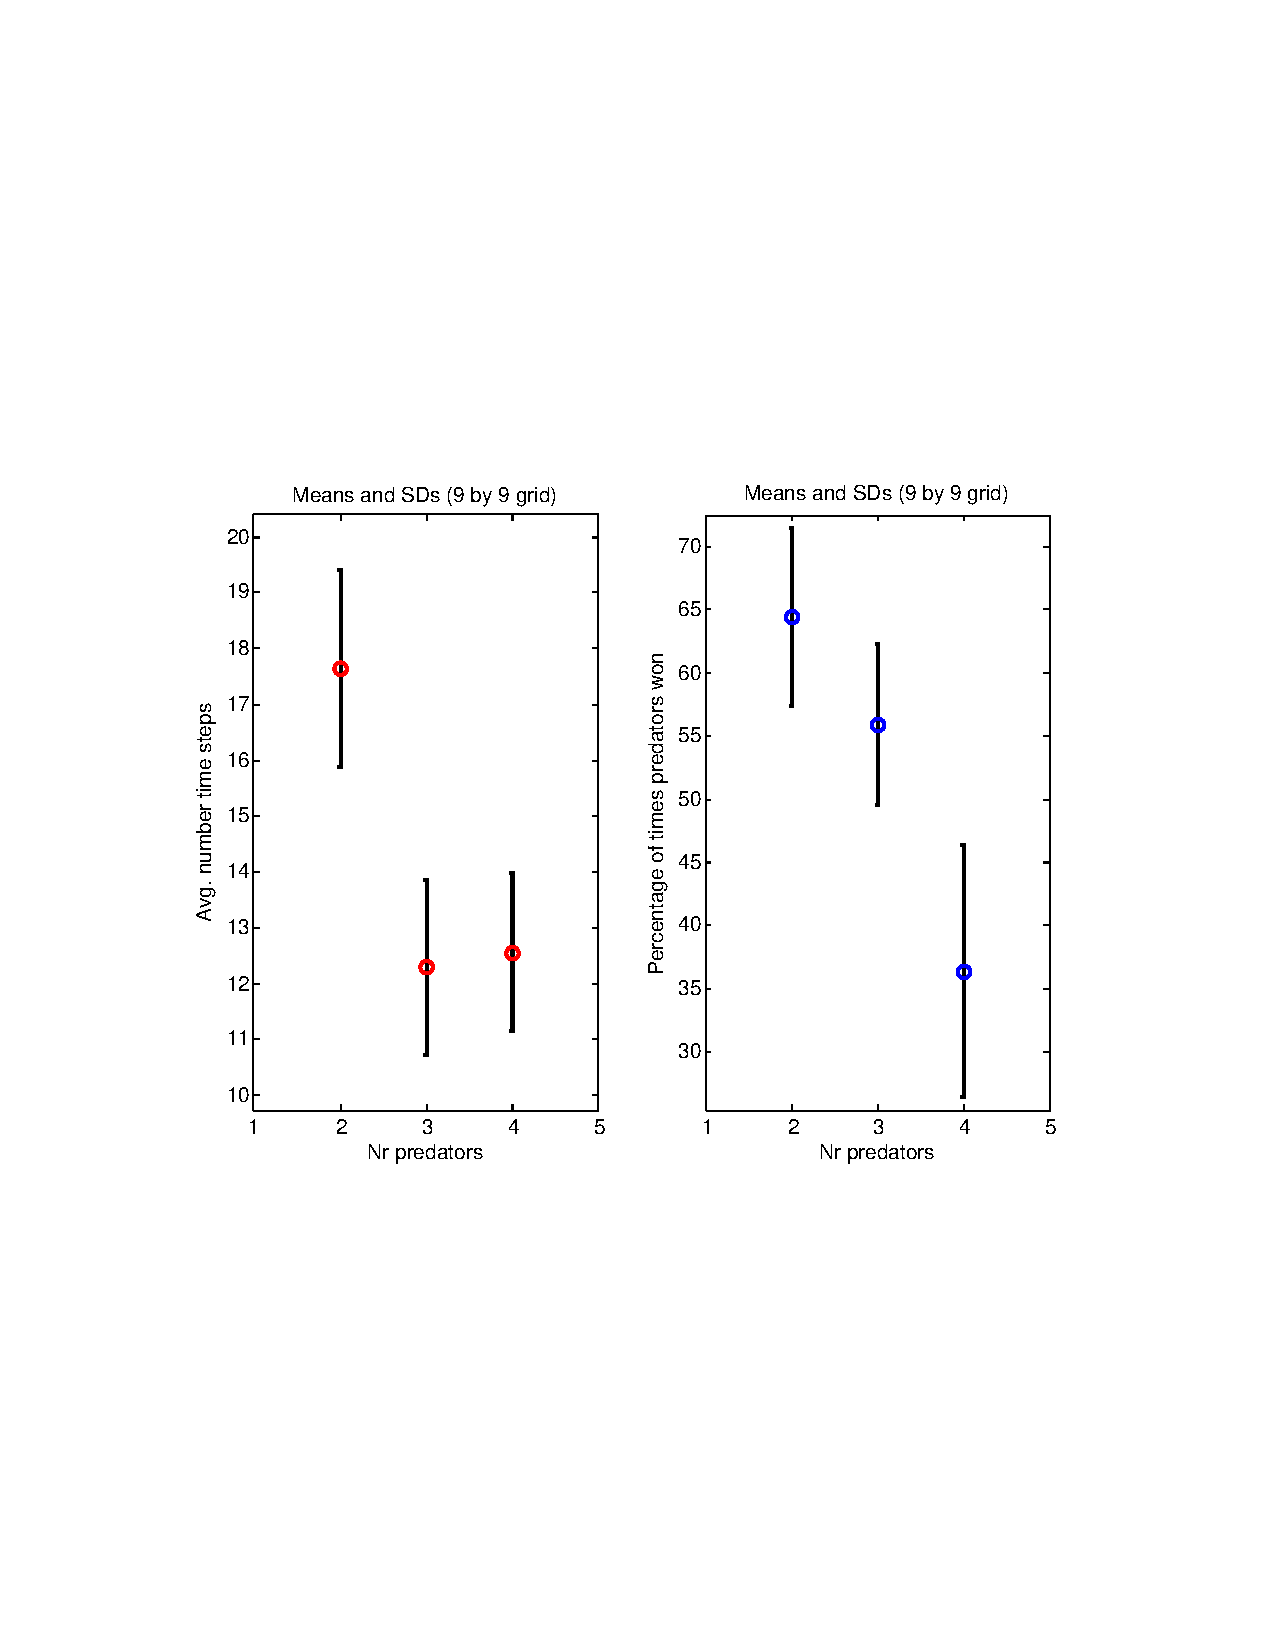
\includegraphics[bb = 0.6in 3in 7.9in 8.5in,clip,width=0.75\textwidth]{IQLgrid9by9ErrorBars.pdf} 
\caption{Means and SD's for performance measures for IQL, for 5000 episodes}
\label{fig:IQLmeansSds}
\end{figure}



We can see that in the case of four predators the percentage of times that the predators won an episode is the smallest. This is probably because of the higher chance of collision and more difficult coordination necessities. The variance for this measure for the case of four predators is also pretty high, also suggesting that a  ``common'' and more or less converged policy is not developed yet (insofar as a true common converged policy is possible under IQL). 

The case of there being three predators performs almost the same as the case of there being four predators on the average number of time steps  needed for termination of an episode. However for the case of there being three predators the episode endings are more often in the predators' favor. It seems, that three predators catch the prey less often than when there are two predators, but they do need less time steps for it.
 
On the other hand, the case of there being two predators performs surprisingly well on the percentage of times the predators won, but needs a lot of time steps for that.

\FloatBarrier

Now it would be interesting to see the performance over time and also if IQL actually converges for these cases, since IQL is not guaranteed to.
In Tables \ref{tab:percentage} and \ref{tab:timeSteps} we show the mean and variance again but now also the last value (i.e. at the $5000\mathrm{th}$ episode, run 200 times) for the corresponding  measure.

\begin{table}[hbt]
\centering
\begin{tabular}{lllll}
 Nr. predators  &  Variance& Mean & Last value   \\ 
\hline   
 2 & 50.109 & 64.482 & 62   \\ 
 3 & 41.104 & 55.941 & 62.5   \\ 
 4 & 99.92  & 36.331 & 60   \\  
\end{tabular} 
\caption{Percentage of times predators won (9 $\times$ 9 grid)}
\label{tab:percentage}
\end{table}

\begin{table}[hbt]
\centering
\begin{tabular}{lllll}
 Nr. predators  &  Variance& Mean & Last value   \\ 
\hline   
 2 &3.08 & 17.64 & 16.61   \\ 
 3 & 2.435 & 12.297 & 12.155   \\ 
 4 & 1.997  & 12.562 & 12.89   \\  
\end{tabular} 
\caption{Average number of time steps  (9 $\times$ 9 grid)}
\label{tab:timeSteps}
\end{table}

We can immediately see that the case of four predators seems to move a large amount up for the measure of the percentage of times they won. Its mean value is 36.331 but its end value is 60. The case for two predators seems to have ``converged'' long before, with a mean close to its last value.

The variance of the case of four predators, for the measure of the percentage of times they won, is quite large.
This can mean the agents either learn very slow or because of large fluctuations in the distribution of ``skill'' over the prey and predators over time. In Figure \ref{fig:IQLpercentagePlot} we show a plot of the percentage of times the predators won for each predator number setting. We indeed see that in the setting of four predators the learning simply occurs slowly.


 In Figure \ref{fig:IQLpercentagePlot} we also see that the predator performance slowly goes down between the 500th and 2000th episode for the case of two predators. Apparently the predators learned to optimize their performance before the prey could, but then the prey learned their policy, and after that escapes more often. The predators apparently can't make a much better policy after that. For the settings of three and four predators, it seems the prey was the first to learn a (up until a certain time) good policy.
 
As for convergence, the average number of time steps used per episode seems to converge for all three settings, as can also be seen in Figure \ref{fig:IQLnrTimeSteps} (and Table \ref{tab:timeSteps}). The percentage of times the predators won, seems to converge for $5000$ episodes only for the settings of two and three predators. The value for four predators seems not stable yet, as can be seen in Figure \ref{fig:IQLpercentagePlot} (and Table \ref{tab:percentage}).



\begin{figure}[htb]
\centering
%bb = llx, lly, urx, and ury;
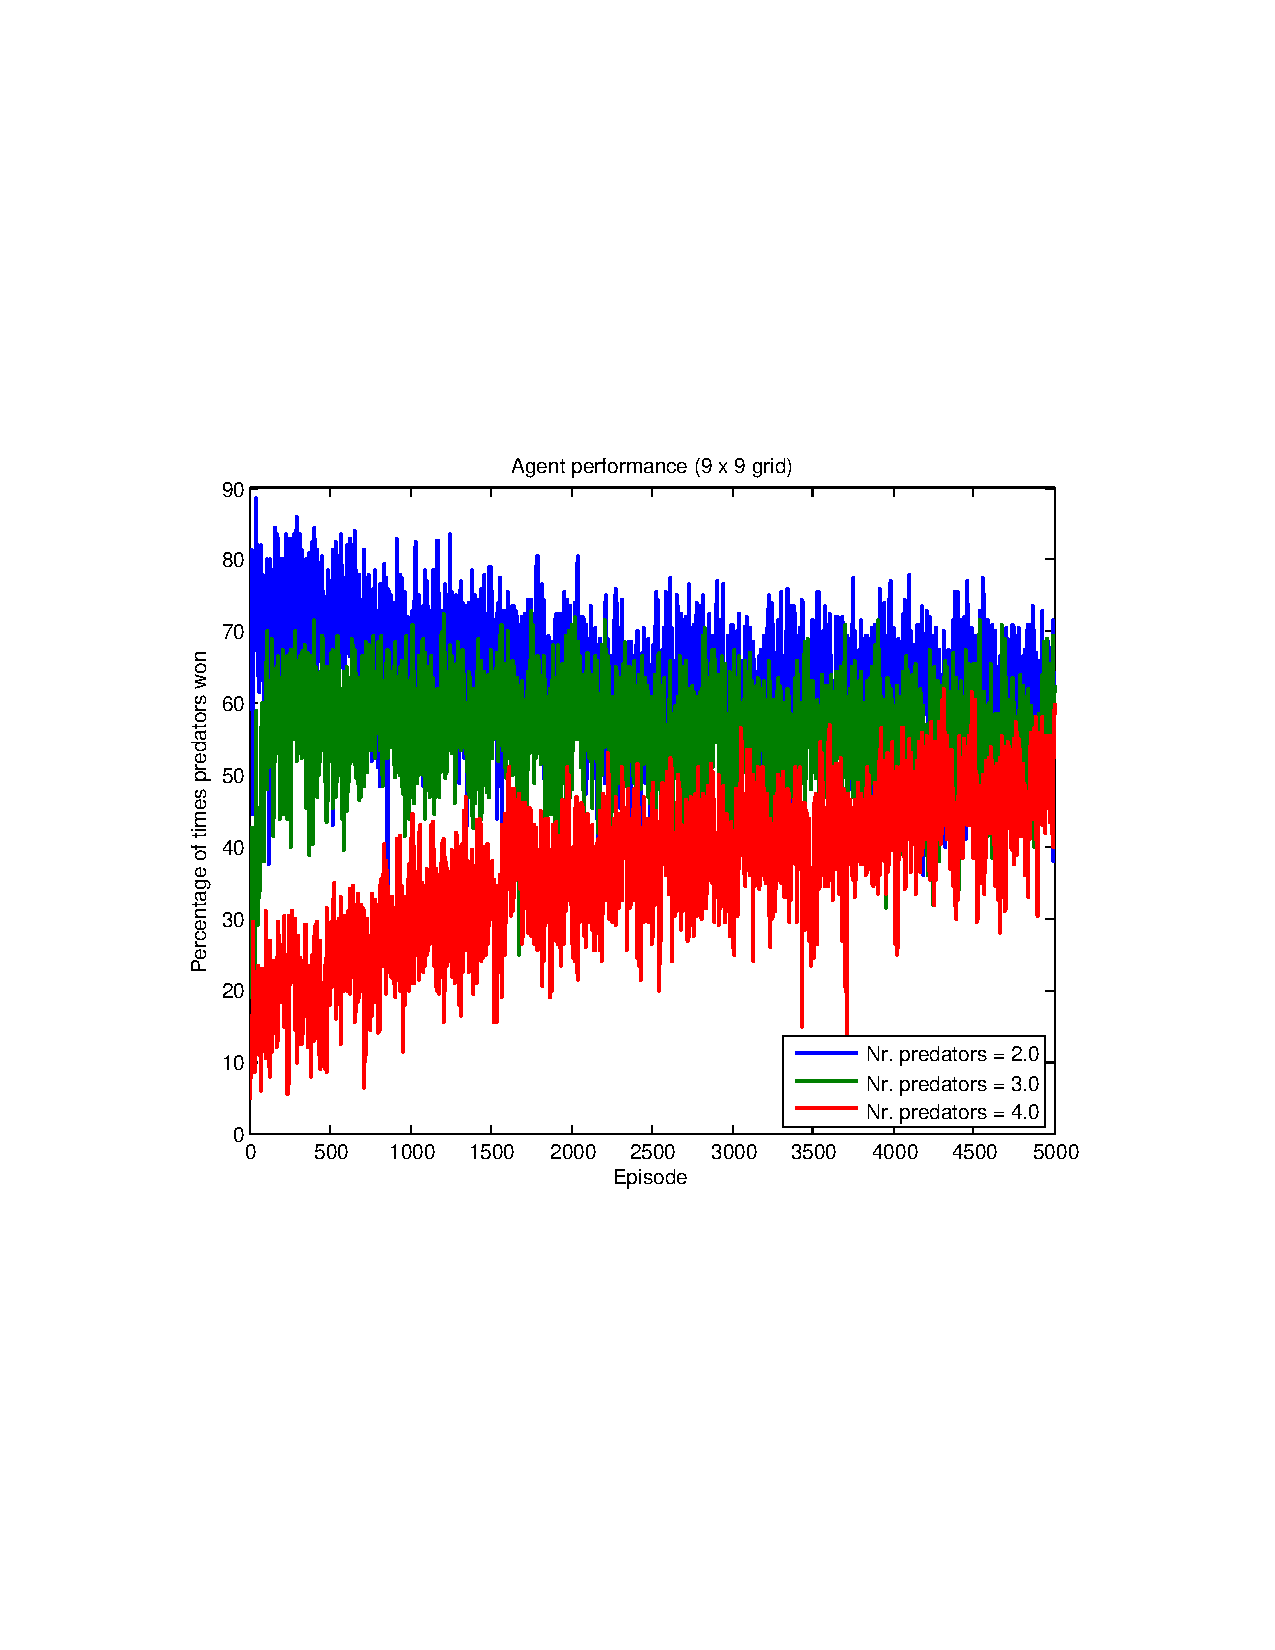
\includegraphics[bb = 0.6in 3in 7.9in 8in,clip,width=0.66\textwidth]
{IQLgrid9by9percentageWinning5000episodesavg200trials.pdf} 
\caption{Percentage of times the predators won for the three predator number settings}
\label{fig:IQLpercentagePlot}
\end{figure}
\begin{figure}[htb]
\centering
%bb = llx, lly, urx, and ury;
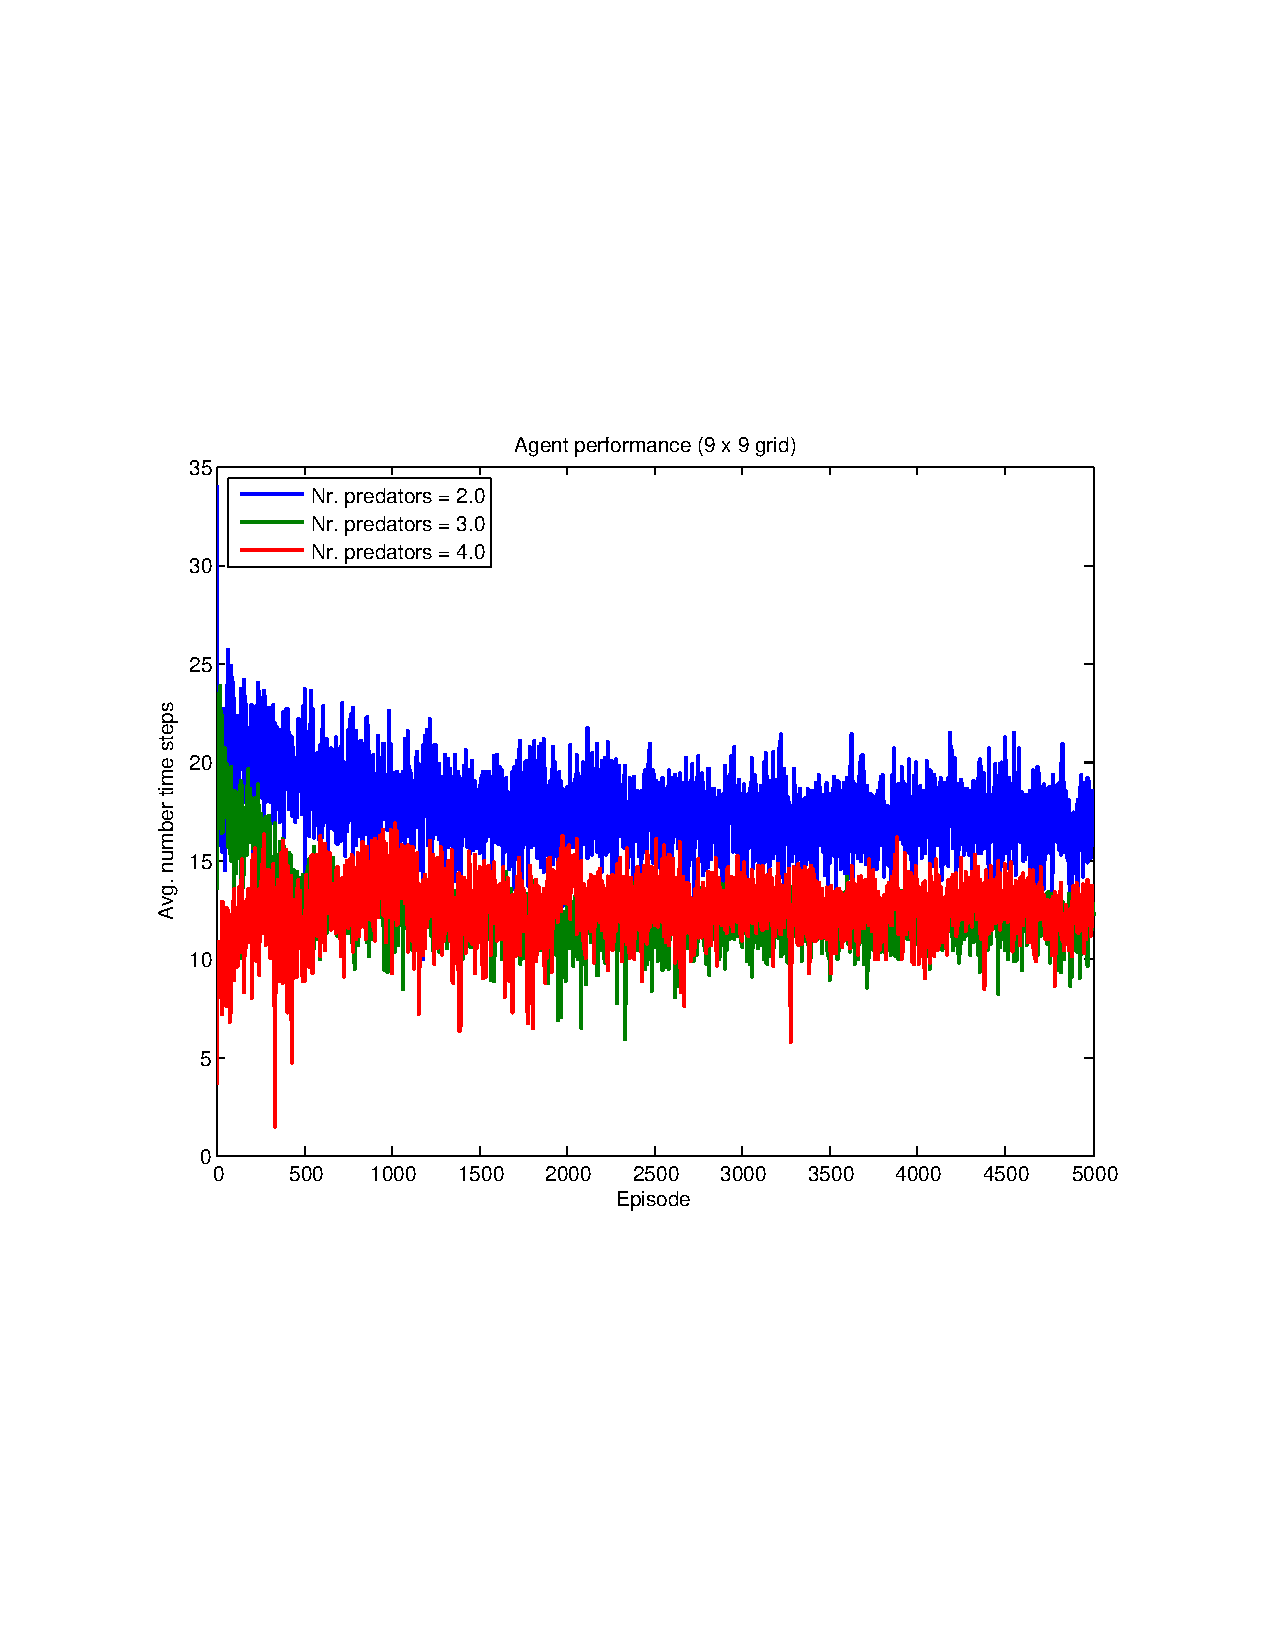
\includegraphics[bb = 0.6in 2.9in 7.9in 8.2in,clip,width=0.66\textwidth]
{IQLgrid9by9nrTimeSteps5000episodesavg200trials.pdf} 
\caption{Average nr. of time steps before an episode ending, for the three predator number settings}
\label{fig:IQLnrTimeSteps}
\end{figure}


\FloatBarrier
\clearpage
\subsubsection{Using an 11 $\times$ 11 grid}

The results for using a larger, $11 \times 11$ grid seem roughly similar to those in Section \ref{sec:IQLresults1} were we used a $9 \times 9$ grid. Compare Figure \ref{fig:IQLpercentagePlot2} with Figure \ref{fig:IQLpercentagePlot} and Figure \ref{fig:IQLnrTimeSteps2} with Figure \ref{fig:IQLnrTimeSteps}. The differences seem more pronounced for the first 1000 episodes. Also, the percentage of times that the predators won, is  higher for the case of three predators in the $11 \times 11$ setting, probably because of less collision issues.

\begin{figure}[hbt]
\centering
%bb = llx, lly, urx, and ury;
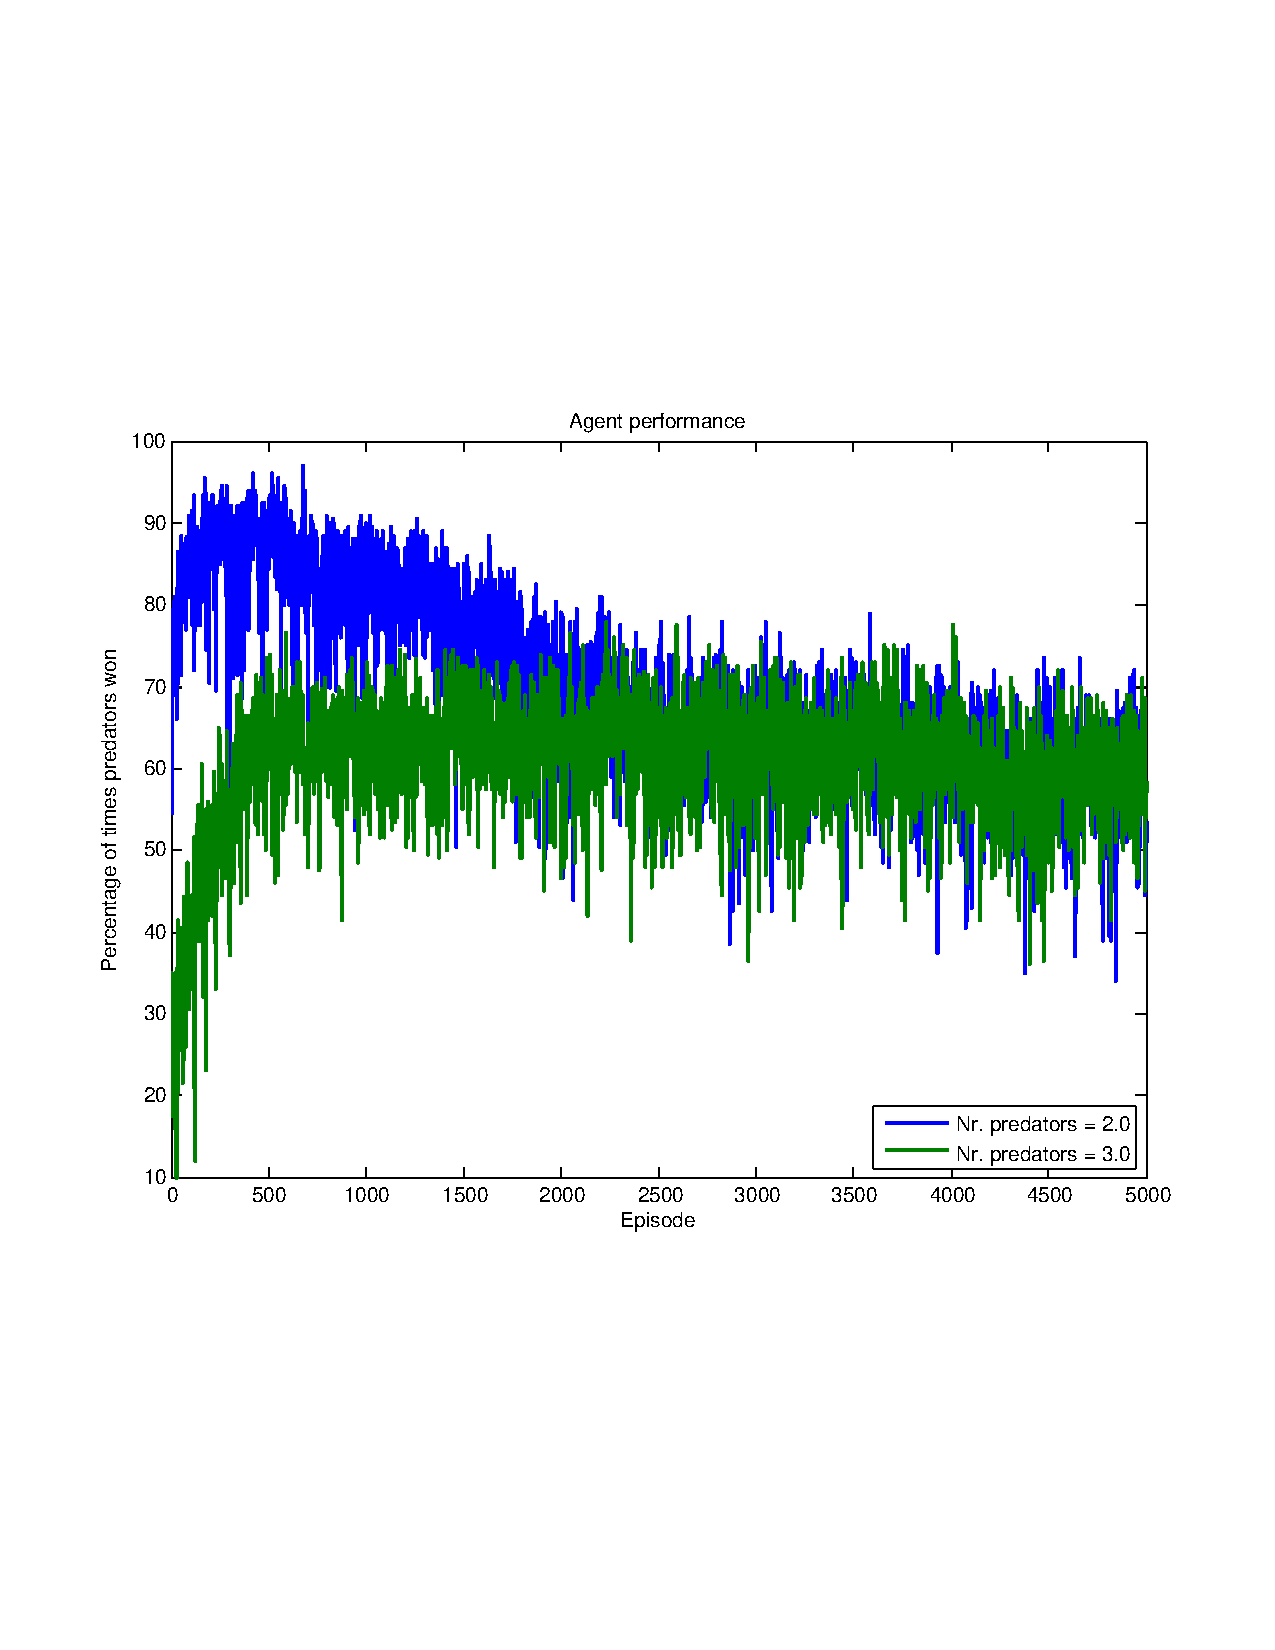
\includegraphics[bb = 0.6in 3in 7.9in 8.3in,clip,width=0.6\textwidth]
{IQLpercentageWinning5000episodesavg200trials.pdf} 
\caption{Percentage of times the predators won for the two predator number settings}
\label{fig:IQLpercentagePlot2}
\end{figure}
\begin{figure}[hbt]
\centering
%bb = llx, lly, urx, and ury;
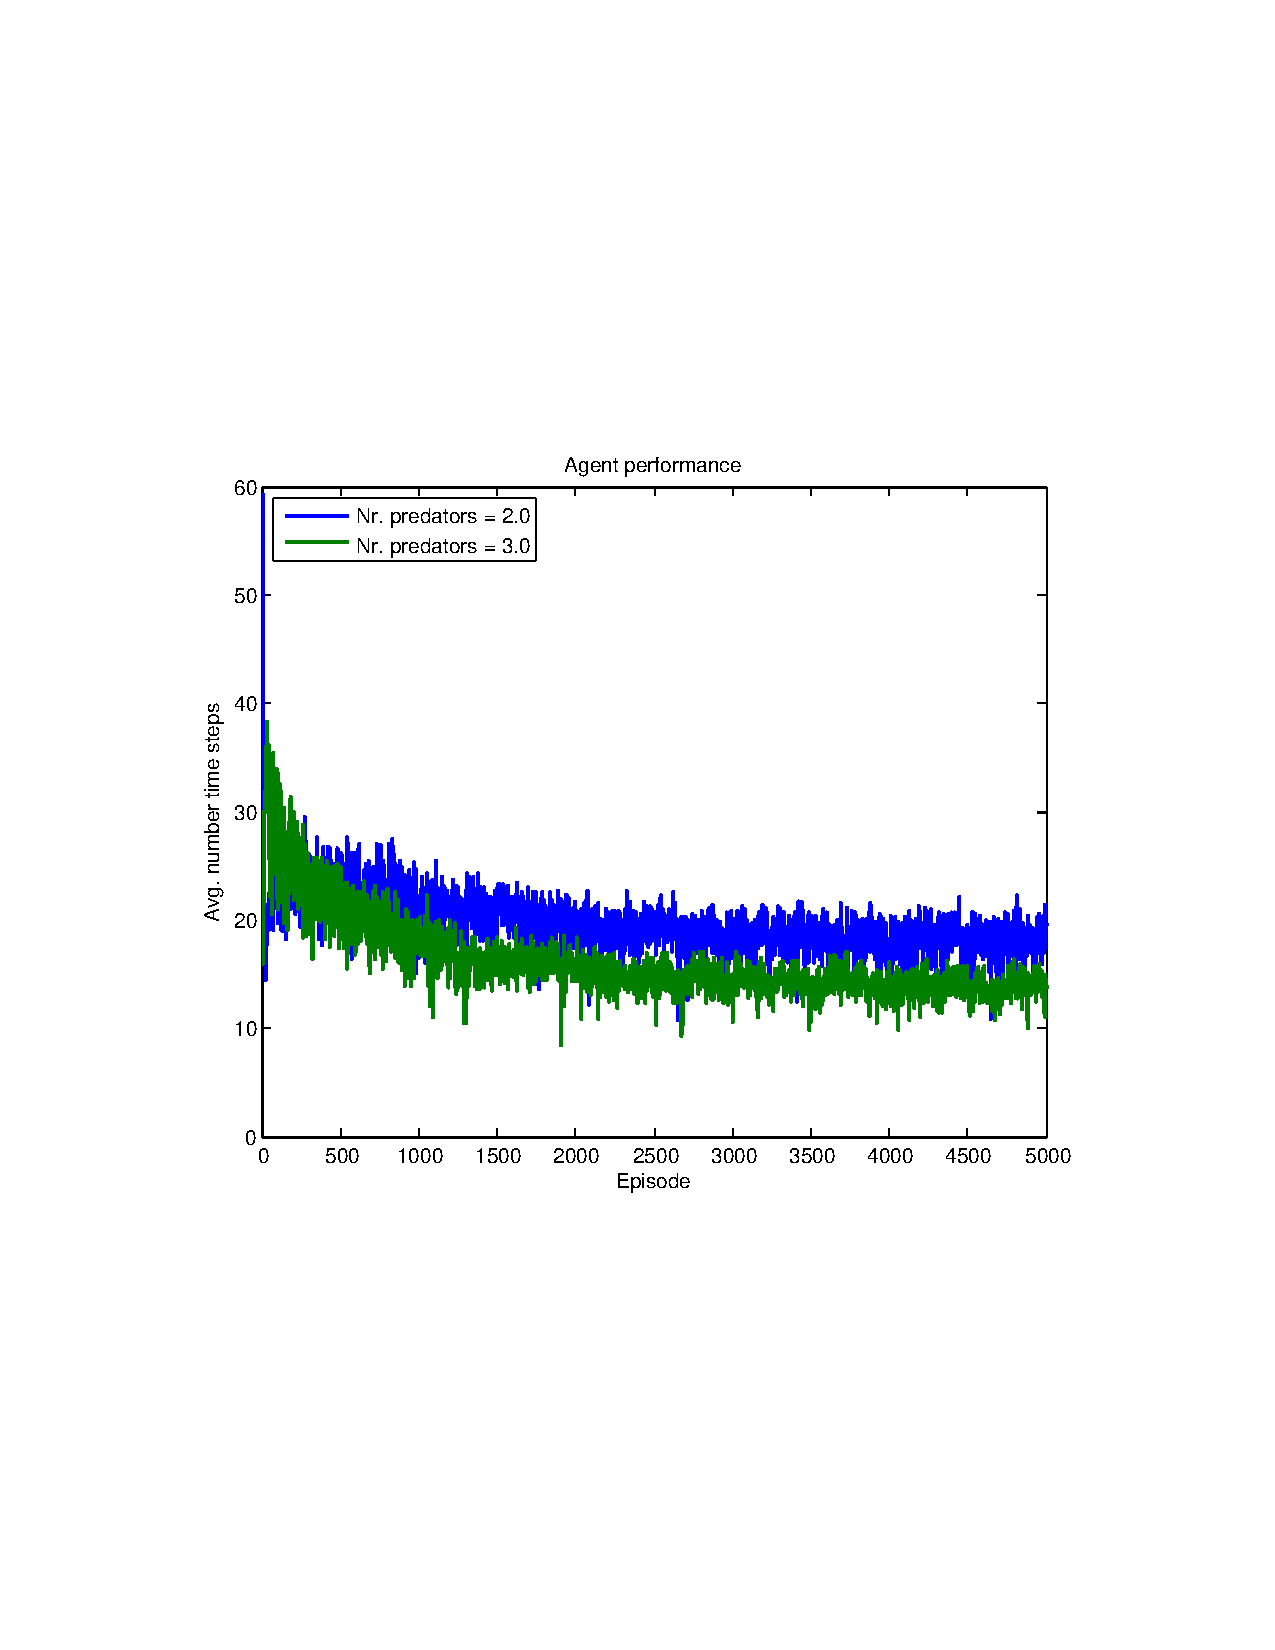
\includegraphics[bb = 0.6in 3in 7.9in 8in,clip,width=0.73\textwidth]{IQLnrTimeSteps5000episodesavg200trials.pdf} 
\caption{Average nr. of time steps before an episode ending, for the two predator number settings}
\label{fig:IQLnrTimeSteps2}
\end{figure}


\clearpage


\section{Minimax-Q algorithm}
The Minimax-Q algorithm can be used for planning in a Markov Game. It is an implementation of the general Minimax principle for Markov Games such as the prey-predator scenario in this assignment. This algorithm needs a strictly competitive scenario and is therefore implemented for the one prey and one predator setting. 

\subsection{Minimax principle and translation to Markov Games}
The Minimax principle is stated in \cite{minimax} as: ``Behave so as to maximize your reward in the worst case''. This means that the policy should be such that the agent takes the action resulting in the highest expected reward under the assumption that the opponent will also take the action that results in the highest expected reward for the opponent.

\noindent The value of a state $s\in S$ in a Markov Game is:
\begin{align*}
V(s) &= \operatorname*{arg\,max}_{\pi \in PD(A)}
\operatorname*{arg\,min}_{o \in O}
\sum_{a \in A} Q(s,a,o) \pi_a
\end{align*}
where
\begin{align*}
Q(s,a,o) &= R(s,a,o) + \gamma \sum_{s'} T(s,a,o,s')V(s')
\end{align*}
Choosing the action that maximizes the reward in the worst case is than the policy that is guaranteed to result in an expected score of $V$ no matter which action the opponent chooses, for the maximal value of $V$. This can be written down in constraints where there is a constraint for each action the opponent can take:
%  
\begin{align*}
\pi_1 \cdot Q(s,a_1,o_1)+ ... + \pi_n \cdot Q(s,a_n,o_1) \geq V\\
\pi_1 \cdot Q(s,a_1,o_2)+ ... + \pi_n \cdot Q(s,a_n,o_2) \geq V\\
...\\
\pi_1 \cdot Q(s,a_1,o_n)+ ... + \pi_n \cdot Q(s,a_n,o_n) \geq V\\
\end{align*}
Of course the probabilities of $\pi$ are bounded by the constraints that they cannot be negative and they need to add up to one. After adding those constraints:

\begin{align*}
\pi_1 + ... + \pi_n &= 1\\
\pi_1 \geq 0\\
...\\
\pi_n  \geq 0\\
\end{align*}
The maximal value for $V$ that can be found for which all constraints hold is stored as $V$ for the next sweep. The resulting values for $\pi$ for each state are the policy used by the agent.

\subsection{Implementation}
The maximal $V$-value for which the constraints above hold can be found using linear programming. For this purpose we used the Linear Programming methods of the JAVA-library Apache Commons Math, which can be found on \cite{commonsmath}. The agent keeps track of a table of $V$-values to be able to calculate $Q(s,a,o)$ in order to find the right values for $\pi$. This can be done a number of times (or sweeps as they are called) as in Value Iteration. The resulting policy is used to behave in the environment to either catch the prey or avoid the predator.

\begin{table}[htb]
\centering
\begin{tabular}{lccccc}
&1&2&3&4&5\\
Minimax Predator vs Random Prey & 9923 & 9432&9517&9545&9572\\
Random Predator vs Minimax Prey & 282& 5000000& 5000000& 5000000& 5000000\\
Minimax Predator vs Minimax Prey & 221& 5000000& 5000000& 5000000& 5000000\\
\end{tabular}
\caption{Number of steps after each sweep for the three matches using a learningrate of 0.8}
\label{tab:minimaxTable}
\end{table}

\FloatBarrier

\subsection{Results}
Three ``matches'' have been held using the Minimax-Q algorithm. The first match is a Random Prey versus a Minimax Predator, the second one a Random Predator versus a Minimax Prey and finally a Minimax Prey versus a Minimax Predator. After each sweep of planning 25 runs in the actual environment are held and the number of steps necessary to catch the prey is recorded. This averaged can then be compared for each sweep and between the different matches. The results for the first five sweeps can be found in \ref{tab:minimaxTable}, the pattern found here does not change when increasing the number of sweeps. The $V$-values for the Minimax Predator can be found in table \ref{tab:predM} and for the Minimax Prey in table \ref{tab:preyM} .  The resulting policies can be found in Appendix \ref{app:policiesM}.

As can be seen in the tables with the $V$-values these look as would be expected based on their definition as described above. For the predator the values increase as the predator is closer to the prey. However for the prey all values are 0. This seems strange but remember that the $V$ values are a linear combination of $Q(s,a,o)$'s and their weights are the corresponding $\pi$'s. In order to maximize the value of $V$ the $\pi$'s that are corresponding to those $Q(s,a,o)$'s that are negative due to the predator catching the prey, will become zero. The maximal reward the prey can have is zero (not getting caught) and therefore the maximal value for $V$ is also zero.  

Unfortunately, the resulting policies make no sense. There are loops present, where the prey or predator keeps jumping forward and backward and the policy does not direct the predator towards the prey or the prey away from the predator. Whether this is due to a bug in the implementation (which we have not been able to find) or to the fact that there are multiple solutions to the constraints above which maximize $V$ is uncertain. If there are multiple solution for two states not all solutions fit necessarily well together, this might cause the bad policies. i.e. for different states the policy might have converged to a different equilibrium.

The effect of this can be found in the number of steps it takes to catch the prey. For the first match, where the Minimax Predator tries to catch the Random Prey, there is no improvement in the number of steps at all. This is due to the resulting policy. For the second match, Random Predator versus Minimax prey, the number of steps needed becomes larger than 5 million (at which point the run is ended due to death of the predator by exhaustion) after the first sweep. The same applies to the third match, Minimax Predator versus Minimax Prey. It is expected that for these two matches the number of steps needed would be larger, since the prey now is an intelligent agent. However, due to the fact that the prey trips one of every five moves, it would be expected that with optimal policies it would take the predator fifty moves to catch the prey. The prey and predator start ten moves apart from each other and each time the prey trips the predator can move in on the prey one move, which happens every five moves, hence fifty moves are approximately needed to catch a Minimax Prey with an optimal policy.  


\begin{table}[htb]
\centering
\begin{tabular}{cccccc}
0,0000 &  &  &  &  & \\
10,0000 & 4,3644 &  &  &  & \\ 
4,3644 & 1,7596 & 0,6019 &  &  & \\
1,7596 & 0,6019 & 0,1624 & 0,0328 &  & \\ 
0,6019 & 0,1624 & 0,0328 & 0,0047 & 0,0005 & \\ 
0,0968 & 0,0328 & 0,0047 & 0,0005 & 0,0000 & 0,0000\\ 
\end{tabular}
\caption{V-values of Minimax Predator using a learningrate of 0.8}
\label{tab:predM}
\end{table}

\begin{table}[htb]
\centering
\begin{tabular}{cccccc}
0,0000 &  &  &  &  & \\ 
0,0000 & 0,0000 &  &  &  & \\ 
0,0000 & 0,0000 & 0,0000 &  &  & \\ 
0,0000 & 0,0000 & 0,0000 & 0,0000 &  & \\ 
0,0000 & 0,0000 & 0,0000 & 0,0000 & 0,0000 & \\ 
0,0000 & 0,0000 & 0,0000 & 0,0000 & 0,0000 & 0,0000\\ 
\end{tabular}
\caption{V-values of Minimax Prey using a learningrate of 0.8}
\label{tab:preyM}
\end{table}

\FloatBarrier

\subsection{Comparison with Independent Q-Learning}\label{sec:comparisonIQLandMinimax}

A policy resulting from Independent Q-Learning (see Section \ref{sec:IQL}) can be compared to a policy found with Minimax-Q for the case in which there is just one predator and one prey. We ran IQL under these settings for 1000 episodes and constructed policies for the predator and the prey. These policies can be found in Appendix \ref{app:policiesIQL} (the corresponding policies for Minimax-Q are in Appendix \ref{app:policiesM}). The number of steps taken by the predator to reach the prey is shown in figure \ref{fig:onePredQLearn}. Comparing the policies of Q-learning and Minimax-Q shows that for the most part they are both straightforward, prey moves away from the predator and the predator moves toward the prey. The exception is the states next to the prey, where Minimax-Q does not move directly towards the prey. The reason is that Minimax-Q responds to the policy of the prey. Q-learning however uses episodic learning and randomness ($\epsilon$-greedy action selection and prey trip chance) to learn the policy. Because of this, Q-learning cannot respond as precise as Minimax-Q. Even though this is true, the average number of time steps needed (150 according to figure \ref{fig:onePredQLearn1000}) to catch the prey is lower for Q-learning than for Minimax-Q as seen in table \ref{tab:minimaxTable}. From this data alone it is not clear why exactly.

\begin{figure}[ht]
\centering
\subfigure[Displays the average number of time steps needed to catch the prey for the first 1000 episodes.]{
    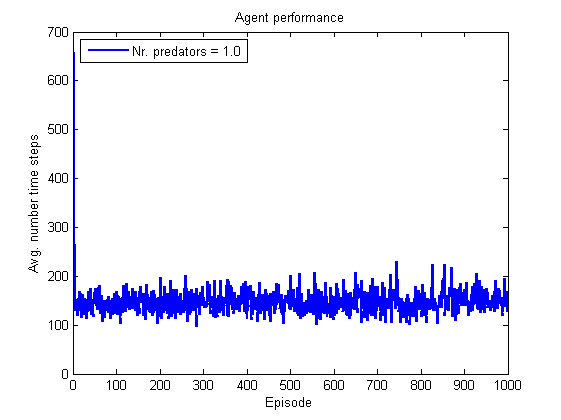
\includegraphics[width=0.45\textwidth]{IQLnrTimeStepsSinglePredator.png}
    \label{fig:onePredQLearn1000}
}
\subfigure[Close-up of figure \ref{fig:onePredQLearn1000}.]{
    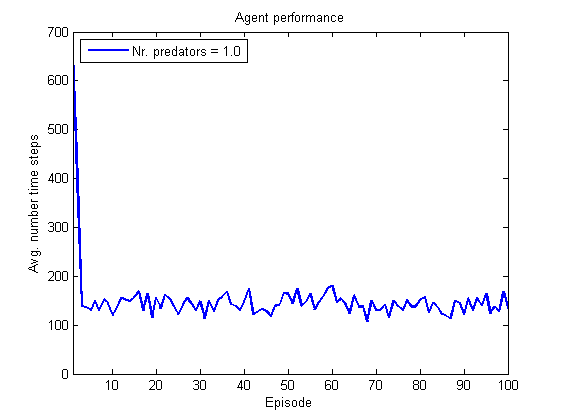
\includegraphics[width=0.45\textwidth]{IQLnrTimeStepsSinglePredatorClose.png}
    \label{fig:onePredQLearnCloseup}
}
\caption{Plots that display the number of time steps needed, averaged over 200 runs for each episode, for a single predator using Q-learning to catch a prey that also uses Q-learning.}
\label{fig:onePredQLearn}
\end{figure}

\section{Conclusion}



\newpage
\appendix
\appendixpage

\section{Class diagram} \label{app:classDiagram}

Hier klassediagram

\section{Policies for Minimax-Q} \label{app:policiesM}
The policies resulting from Minimax-Q can be found in table \ref{policyLabelPred} for the predator and in table \ref{policyLabelPrey} for the prey.

\begin{table}[htbp]
\caption{Policy resulting from Minimax-Q for the predator}
\label{policyLabelPred}
\centering
\begin{footnotesize}
\begin{tabular}{c|c|c|c|c|c|c|c|c|c|c|c|}
&0&1&2&3&4&5&6&7&8&9&10\\ \hline\\
0&U 0,000&U 0,000&U 0,000&U 0,000&U 0,000&U 0,000&U 0,000&U 0,000&U 0,000&U 0,000&U 0,000\\
&R 1,000&R 1,000&R 1,000&R 1,000&R 0,000&R 0,000&R 0,000&R 0,000&R 0,000&R 0,000&R 0,000\\
&D 0,000&D 0,000&D 0,000&D 0,000&D 1,000&D 1,000&D 1,000&D 0,000&D 0,000&D 0,000&D 0,000\\
&L 0,000&L 0,000&L 0,000&L 0,000&L 0,000&L 0,000&L 0,000&L 1,000&L 1,000&L 1,000&L 1,000\\
&W 0,000&W 0,000&W 0,000&W 0,000&W 0,000&W 0,000&W 0,000&W 0,000&W 0,000&W 0,000&W 0,000\\
\hline \\
1&U 0,000&U 0,000&U 0,000&U 0,000&U 0,000&U 0,000&U 0,000&U 0,000&U 0,000&U 0,000&U 0,000\\
&R 0,000&R 1,000&R 1,000&R 1,000&R 0,000&R 0,000&R 0,000&R 0,000&R 0,000&R 0,000&R 0,000\\
&D 1,000&D 0,000&D 0,000&D 0,000&D 1,000&D 1,000&D 1,000&D 0,000&D 0,000&D 0,000&D 0,000\\
&L 0,000&L 0,000&L 0,000&L 0,000&L 0,000&L 0,000&L 0,000&L 1,000&L 1,000&L 1,000&L 1,000\\
&W 0,000&W 0,000&W 0,000&W 0,000&W 0,000&W 0,000&W 0,000&W 0,000&W 0,000&W 0,000&W 0,000\\
\hline \\
2&U 0,000&U 0,000&U 0,000&U 0,000&U 0,000&U 0,000&U 0,000&U 0,000&U 0,000&U 0,000&U 0,000\\
&R 0,000&R 0,000&R 1,000&R 1,000&R 1,000&R 0,000&R 0,000&R 0,000&R 0,000&R 0,000&R 0,000\\
&D 1,000&D 1,000&D 0,000&D 0,000&D 0,000&D 1,000&D 0,000&D 0,000&D 0,000&D 0,000&D 1,000\\
&L 0,000&L 0,000&L 0,000&L 0,000&L 0,000&L 0,000&L 1,000&L 1,000&L 1,000&L 1,000&L 0,000\\
&W 0,000&W 0,000&W 0,000&W 0,000&W 0,000&W 0,000&W 0,000&W 0,000&W 0,000&W 0,000&W 0,000\\
\hline \\
3&U 0,000&U 0,000&U 0,000&U 0,000&U 0,000&U 0,000&U 0,000&U 0,000&U 0,000&U 0,000&U 0,000\\
&R 0,000&R 0,000&R 0,000&R 1,000&R 1,000&R 0,000&R 0,000&R 0,000&R 0,000&R 0,000&R 0,000\\
&D 1,000&D 1,000&D 1,000&D 0,000&D 0,000&D 1,000&D 0,000&D 0,000&D 0,000&D 1,000&D 1,000\\
&L 0,000&L 0,000&L 0,000&L 0,000&L 0,000&L 0,000&L 1,000&L 1,000&L 1,000&L 0,000&L 0,000\\
&W 0,000&W 0,000&W 0,000&W 0,000&W 0,000&W 0,000&W 0,000&W 0,000&W 0,000&W 0,000&W 0,000\\
\hline \\
4&U 0,000&U 0,000&U 0,000&U 0,000&U 0,000&U 0,000&U 0,000&U 0,000&U 0,000&U 0,000&U 0,000\\
&R 1,000&R 1,000&R 0,000&R 0,000&R 1,000&R 1,000&R 0,000&R 0,000&R 0,000&R 0,000&R 0,000\\
&D 0,000&D 0,000&D 1,000&D 1,000&D 0,000&D 0,000&D 0,000&D 0,000&D 1,000&D 0,000&D 0,000\\
&L 0,000&L 0,000&L 0,000&L 0,000&L 0,000&L 0,000&L 1,000&L 1,000&L 0,000&L 1,000&L 1,000\\
&W 0,000&W 0,000&W 0,000&W 0,000&W 0,000&W 0,000&W 0,000&W 0,000&W 0,000&W 0,000&W 0,000\\
\hline \\
5&U 0,000&U 0,000&U 0,000&U 0,000&U 0,000&&U 0,000&U 0,000&U 0,000&U 0,000&U 0,000\\
&R 1,000&R 1,000&R 1,000&R 1,000&R 0,000&&R 0,000&R 0,000&R 0,000&R 0,000&R 0,000\\
&D 0,000&D 0,000&D 0,000&D 0,000&D 1,000&Prey&D 0,000&D 0,000&D 0,000&D 0,000&D 0,000\\
&L 0,000&L 0,000&L 0,000&L 0,000&L 0,000&&L 1,000&L 1,000&L 1,000&L 1,000&L 1,000\\
&W 0,000&W 0,000&W 0,000&W 0,000&W 0,000&&W 0,000&W 0,000&W 0,000&W 0,000&W 0,000\\
\hline \\
6&U 0,000&U 0,000&U 1,000&U 1,000&U 1,000&U 0,000&U 1,000&U 1,000&U 1,000&U 0,000&U 0,000\\
&R 1,000&R 1,000&R 0,000&R 0,000&R 0,000&R 1,000&R 0,000&R 0,000&R 0,000&R 0,000&R 0,000\\
&D 0,000&D 0,000&D 0,000&D 0,000&D 0,000&D 0,000&D 0,000&D 0,000&D 0,000&D 0,000&D 0,000\\
&L 0,000&L 0,000&L 0,000&L 0,000&L 0,000&L 0,000&L 0,000&L 0,000&L 0,000&L 1,000&L 1,000\\
&W 0,000&W 0,000&W 0,000&W 0,000&W 0,000&W 0,000&W 0,000&W 0,000&W 0,000&W 0,000&W 0,000\\
\hline \\
7&U 1,000&U 1,000&U 1,000&U 1,000&U 0,000&U 1,000&U 0,000&U 1,000&U 1,000&U 1,000&U 1,000\\
&R 0,000&R 0,000&R 0,000&R 0,000&R 1,000&R 0,000&R 0,000&R 0,000&R 0,000&R 0,000&R 0,000\\
&D 0,000&D 0,000&D 0,000&D 0,000&D 0,000&D 0,000&D 0,000&D 0,000&D 0,000&D 0,000&D 0,000\\
&L 0,000&L 0,000&L 0,000&L 0,000&L 0,000&L 0,000&L 1,000&L 0,000&L 0,000&L 0,000&L 0,000\\
&W 0,000&W 0,000&W 0,000&W 0,000&W 0,000&W 0,000&W 0,000&W 0,000&W 0,000&W 0,000&W 0,000\\
\hline \\
8&U 1,000&U 1,000&U 1,000&U 0,000&U 0,000&U 1,000&U 0,000&U 0,000&U 1,000&U 1,000&U 1,000\\
&R 0,000&R 0,000&R 0,000&R 1,000&R 1,000&R 0,000&R 0,000&R 0,000&R 0,000&R 0,000&R 0,000\\
&D 0,000&D 0,000&D 0,000&D 0,000&D 0,000&D 0,000&D 0,000&D 0,000&D 0,000&D 0,000&D 0,000\\
&L 0,000&L 0,000&L 0,000&L 0,000&L 0,000&L 0,000&L 1,000&L 1,000&L 0,000&L 0,000&L 0,000\\
&W 0,000&W 0,000&W 0,000&W 0,000&W 0,000&W 0,000&W 0,000&W 0,000&W 0,000&W 0,000&W 0,000\\
\hline \\
9&U 1,000&U 1,000&U 0,000&U 0,000&U 1,000&U 1,000&U 1,000&U 0,000&U 0,000&U 1,000&U 1,000\\
&R 0,000&R 0,000&R 1,000&R 1,000&R 0,000&R 0,000&R 0,000&R 0,000&R 0,000&R 0,000&R 0,000\\
&D 0,000&D 0,000&D 0,000&D 0,000&D 0,000&D 0,000&D 0,000&D 0,000&D 0,000&D 0,000&D 0,000\\
&L 0,000&L 0,000&L 0,000&L 0,000&L 0,000&L 0,000&L 0,000&L 1,000&L 1,000&L 0,000&L 0,000\\
&W 0,000&W 0,000&W 0,000&W 0,000&W 0,000&W 0,000&W 0,000&W 0,000&W 0,000&W 0,000&W 0,000\\
\hline \\
10&U 1,000&U 0,000&U 0,000&U 0,000&U 1,000&U 1,000&U 1,000&U 0,000&U 0,000&U 0,000&U 1,000\\
&R 0,000&R 1,000&R 1,000&R 1,000&R 0,000&R 0,000&R 0,000&R 0,000&R 0,000&R 0,000&R 0,000\\
&D 0,000&D 0,000&D 0,000&D 0,000&D 0,000&D 0,000&D 0,000&D 0,000&D 0,000&D 0,000&D 0,000\\
&L 0,000&L 0,000&L 0,000&L 0,000&L 0,000&L 0,000&L 0,000&L 1,000&L 1,000&L 1,000&L 0,000\\
&W 0,000&W 0,000&W 0,000&W 0,000&W 0,000&W 0,000&W 0,000&W 0,000&W 0,000&W 0,000&W 0,000\\
\hline \\
\end{tabular}
\end{footnotesize}
\end{table}


 \begin{table}[htbp]
\caption{Policy resulting from Minimax-Q for the prey}
\label{policyLabelPrey}
\centering
\begin{footnotesize}
\begin{tabular}{c|c|c|c|c|c|c|c|c|c|c|c|}
&0&1&2&3&4&5&6&7&8&9&10\\ \hline\\
0&U 0,000&U 0,000&U 0,000&U 0,000&U 0,000&U 0,000&U 0,000&U 0,000&U 0,000&U 0,000&U 0,000\\
&R 1,000&R 1,000&R 1,000&R 1,000&R 1,000&R 1,000&R 0,000&R 0,000&R 0,000&R 0,000&R 0,000\\
&D 0,000&D 0,000&D 0,000&D 0,000&D 0,000&D 0,000&D 0,000&D 0,000&D 0,000&D 0,000&D 0,000\\
&L 0,000&L 0,000&L 0,000&L 0,000&L 0,000&L 0,000&L 1,000&L 1,000&L 1,000&L 1,000&L 1,000\\
&W 0,000&W 0,000&W 0,000&W 0,000&W 0,000&W 0,000&W 0,000&W 0,000&W 0,000&W 0,000&W 0,000\\
\hline \\
1&U 0,000&U 0,000&U 0,000&U 0,000&U 0,000&U 0,000&U 0,000&U 0,000&U 0,000&U 0,000&U 0,000\\
&R 0,000&R 1,000&R 1,000&R 1,000&R 1,000&R 1,000&R 0,000&R 0,000&R 0,000&R 0,000&R 0,000\\
&D 1,000&D 0,000&D 0,000&D 0,000&D 0,000&D 0,000&D 0,000&D 0,000&D 0,000&D 0,000&D 0,000\\
&L 0,000&L 0,000&L 0,000&L 0,000&L 0,000&L 0,000&L 1,000&L 1,000&L 1,000&L 1,000&L 1,000\\
&W 0,000&W 0,000&W 0,000&W 0,000&W 0,000&W 0,000&W 0,000&W 0,000&W 0,000&W 0,000&W 0,000\\
\hline \\
2&U 0,000&U 0,000&U 0,000&U 0,000&U 0,000&U 0,000&U 0,000&U 0,000&U 0,000&U 0,000&U 0,000\\
&R 0,000&R 0,000&R 1,000&R 1,000&R 1,000&R 1,000&R 0,000&R 0,000&R 0,000&R 0,000&R 0,000\\
&D 1,000&D 1,000&D 0,000&D 0,000&D 0,000&D 0,000&D 0,000&D 0,000&D 0,000&D 0,000&D 1,000\\
&L 0,000&L 0,000&L 0,000&L 0,000&L 0,000&L 0,000&L 1,000&L 1,000&L 1,000&L 1,000&L 0,000\\
&W 0,000&W 0,000&W 0,000&W 0,000&W 0,000&W 0,000&W 0,000&W 0,000&W 0,000&W 0,000&W 0,000\\
\hline \\
3&U 0,000&U 0,000&U 0,000&U 0,000&U 0,000&U 0,000&U 0,000&U 0,000&U 0,000&U 0,000&U 0,000\\
&R 0,000&R 0,000&R 0,000&R 1,000&R 1,000&R 1,000&R 0,000&R 0,000&R 0,000&R 0,000&R 0,000\\
&D 1,000&D 1,000&D 1,000&D 0,000&D 0,000&D 0,000&D 0,000&D 0,000&D 0,000&D 1,000&D 1,000\\
&L 0,000&L 0,000&L 0,000&L 0,000&L 0,000&L 0,000&L 1,000&L 1,000&L 1,000&L 0,000&L 0,000\\
&W 0,000&W 0,000&W 0,000&W 0,000&W 0,000&W 0,000&W 0,000&W 0,000&W 0,000&W 0,000&W 0,000\\
\hline \\
4&U 0,000&U 0,000&U 0,000&U 0,000&U 0,000&U 0,000&U 0,000&U 0,000&U 0,000&U 0,000&U 0,000\\
&R 0,000&R 0,000&R 0,000&R 0,000&R 1,000&R 1,000&R 0,000&R 0,000&R 0,000&R 0,000&R 0,000\\
&D 1,000&D 1,000&D 1,000&D 1,000&D 0,000&D 0,000&D 0,000&D 0,000&D 1,000&D 1,000&D 1,000\\
&L 0,000&L 0,000&L 0,000&L 0,000&L 0,000&L 0,000&L 1,000&L 1,000&L 0,000&L 0,000&L 0,000\\
&W 0,000&W 0,000&W 0,000&W 0,000&W 0,000&W 0,000&W 0,000&W 0,000&W 0,000&W 0,000&W 0,000\\
\hline \\
5&U 0,000&U 0,000&U 0,000&U 0,000&U 0,000&&U 0,000&U 0,000&U 0,000&U 0,000&U 0,000\\
&R 0,000&R 0,000&R 0,000&R 0,000&R 0,000&&R 0,000&R 0,000&R 0,000&R 0,000&R 0,000\\
&D 1,000&D 1,000&D 1,000&D 1,000&D 1,000&Pred&D 0,000&D 1,000&D 1,000&D 1,000&D 1,000\\
&L 0,000&L 0,000&L 0,000&L 0,000&L 0,000&&L 1,000&L 0,000&L 0,000&L 0,000&L 0,000\\
&W 0,000&W 0,000&W 0,000&W 0,000&W 0,000&&W 0,000&W 0,000&W 0,000&W 0,000&W 0,000\\
\hline \\
6&U 1,000&U 1,000&U 1,000&U 1,000&U 1,000&U 0,000&U 1,000&U 1,000&U 1,000&U 1,000&U 1,000\\
&R 0,000&R 0,000&R 0,000&R 0,000&R 0,000&R 1,000&R 0,000&R 0,000&R 0,000&R 0,000&R 0,000\\
&D 0,000&D 0,000&D 0,000&D 0,000&D 0,000&D 0,000&D 0,000&D 0,000&D 0,000&D 0,000&D 0,000\\
&L 0,000&L 0,000&L 0,000&L 0,000&L 0,000&L 0,000&L 0,000&L 0,000&L 0,000&L 0,000&L 0,000\\
&W 0,000&W 0,000&W 0,000&W 0,000&W 0,000&W 0,000&W 0,000&W 0,000&W 0,000&W 0,000&W 0,000\\
\hline \\
7&U 1,000&U 1,000&U 1,000&U 1,000&U 0,000&U 0,000&U 0,000&U 1,000&U 1,000&U 1,000&U 1,000\\
&R 0,000&R 0,000&R 0,000&R 0,000&R 1,000&R 1,000&R 0,000&R 0,000&R 0,000&R 0,000&R 0,000\\
&D 0,000&D 0,000&D 0,000&D 0,000&D 0,000&D 0,000&D 0,000&D 0,000&D 0,000&D 0,000&D 0,000\\
&L 0,000&L 0,000&L 0,000&L 0,000&L 0,000&L 0,000&L 1,000&L 0,000&L 0,000&L 0,000&L 0,000\\
&W 0,000&W 0,000&W 0,000&W 0,000&W 0,000&W 0,000&W 0,000&W 0,000&W 0,000&W 0,000&W 0,000\\
\hline \\
8&U 1,000&U 1,000&U 1,000&U 0,000&U 0,000&U 0,000&U 0,000&U 0,000&U 1,000&U 1,000&U 1,000\\
&R 0,000&R 0,000&R 0,000&R 1,000&R 1,000&R 1,000&R 0,000&R 0,000&R 0,000&R 0,000&R 0,000\\
&D 0,000&D 0,000&D 0,000&D 0,000&D 0,000&D 0,000&D 0,000&D 0,000&D 0,000&D 0,000&D 0,000\\
&L 0,000&L 0,000&L 0,000&L 0,000&L 0,000&L 0,000&L 1,000&L 1,000&L 0,000&L 0,000&L 0,000\\
&W 0,000&W 0,000&W 0,000&W 0,000&W 0,000&W 0,000&W 0,000&W 0,000&W 0,000&W 0,000&W 0,000\\
\hline \\
9&U 1,000&U 1,000&U 0,000&U 0,000&U 0,000&U 0,000&U 0,000&U 0,000&U 0,000&U 1,000&U 1,000\\
&R 0,000&R 0,000&R 1,000&R 1,000&R 1,000&R 1,000&R 0,000&R 0,000&R 0,000&R 0,000&R 0,000\\
&D 0,000&D 0,000&D 0,000&D 0,000&D 0,000&D 0,000&D 0,000&D 0,000&D 0,000&D 0,000&D 0,000\\
&L 0,000&L 0,000&L 0,000&L 0,000&L 0,000&L 0,000&L 1,000&L 1,000&L 1,000&L 0,000&L 0,000\\
&W 0,000&W 0,000&W 0,000&W 0,000&W 0,000&W 0,000&W 0,000&W 0,000&W 0,000&W 0,000&W 0,000\\
\hline \\
10&U 1,000&U 0,000&U 0,000&U 0,000&U 0,000&U 0,000&U 0,000&U 0,000&U 0,000&U 0,000&U 1,000\\
&R 0,000&R 1,000&R 1,000&R 1,000&R 1,000&R 1,000&R 0,000&R 0,000&R 0,000&R 0,000&R 0,000\\
&D 0,000&D 0,000&D 0,000&D 0,000&D 0,000&D 0,000&D 0,000&D 0,000&D 0,000&D 0,000&D 0,000\\
&L 0,000&L 0,000&L 0,000&L 0,000&L 0,000&L 0,000&L 1,000&L 1,000&L 1,000&L 1,000&L 0,000\\
&W 0,000&W 0,000&W 0,000&W 0,000&W 0,000&W 0,000&W 0,000&W 0,000&W 0,000&W 0,000&W 0,000\\
\hline \\
\end{tabular}
\end{footnotesize}
\end{table}

\newpage
\nocite{*}
\bibliographystyle{plainnat}
\bibliography{references}
\begin{thebibliography}{9}

\bibitem{minimax}
  M.L. Littman,
  \emph{Markov games as a framework for multi-agent reinforcement learning}. In Proceedings of the Eleventh International Conference on Machine Learning, pp. 157-163 San Francisco, CA. Morgan Kaufmann.(1994).
  
\end{thebibliography}
\end{document}



\end{document}